%*****************************************
\chapter{Stand der Forschung}\label{ch:relatedWork}
%*****************************************

\section{Die Ontologie: SNIK}

Das Semantische Netz des Informationsmanagements im Krankenhaus (SNIK) ist eine die Domäne des Informationsmanagements im Krankenhaus betreffende Ontologie.
Sie behandelt,
\todo{SNIK}

\begin{sidewaysfigure}[htbp!]
\centering
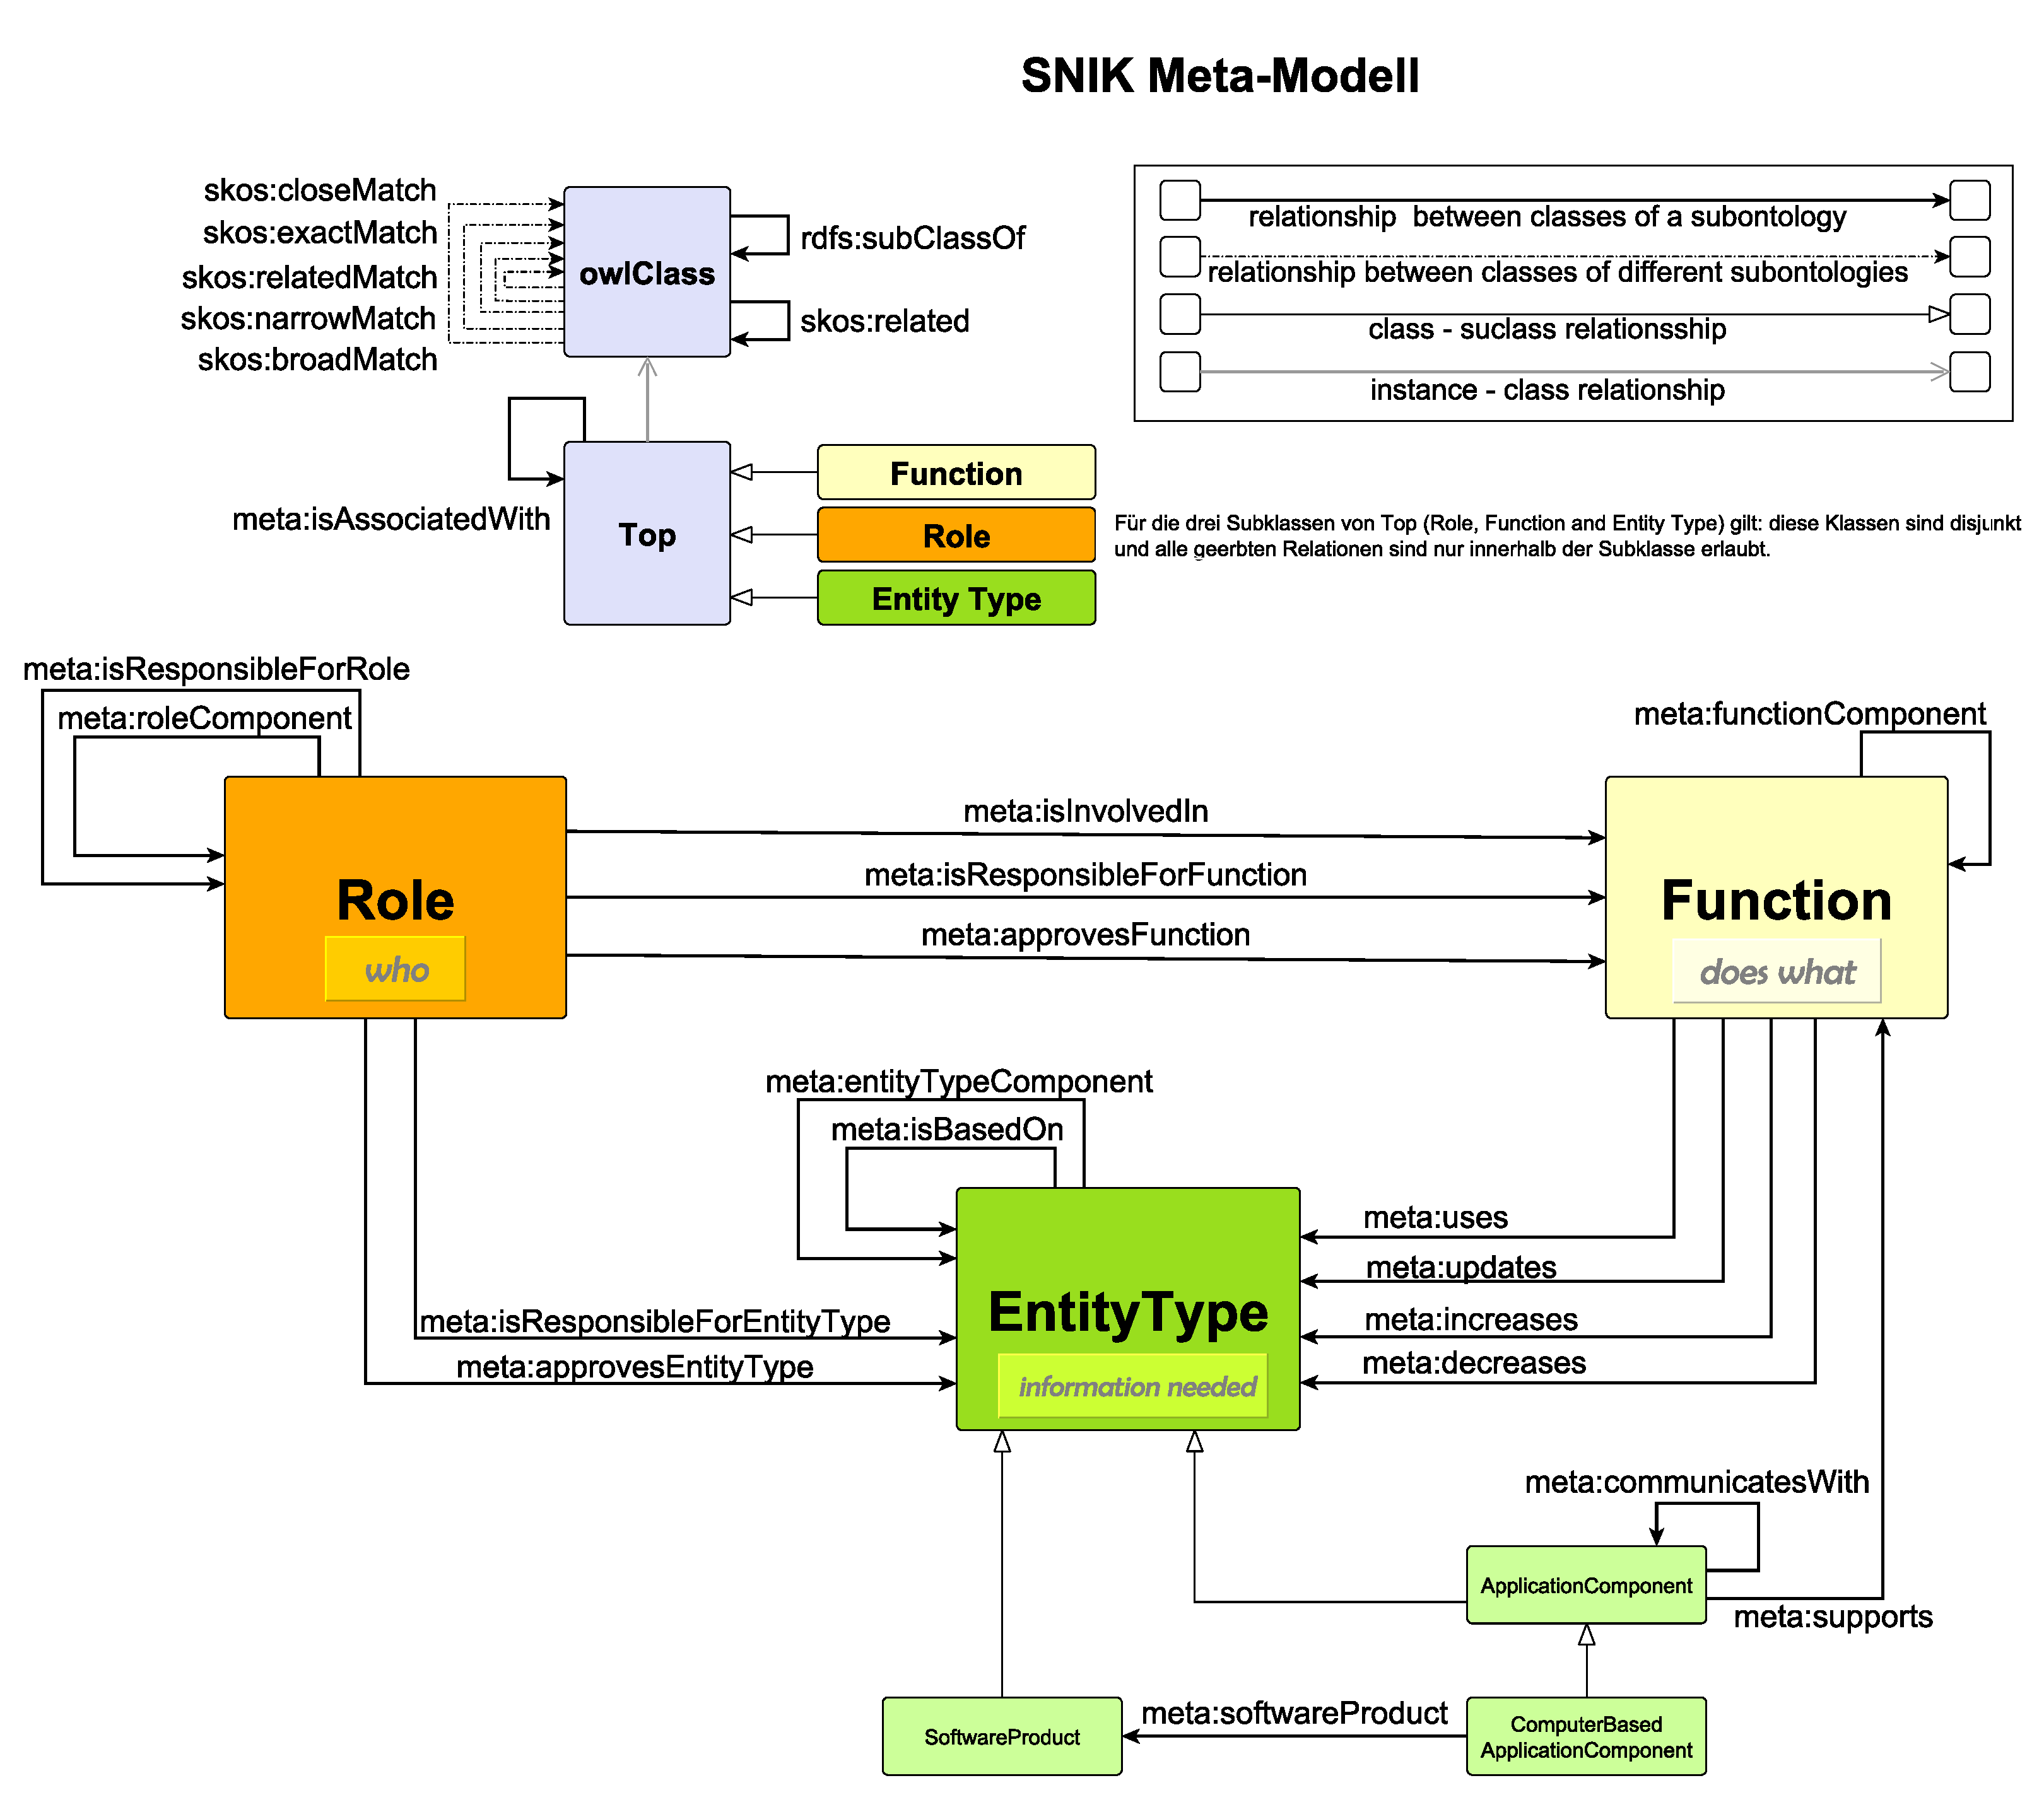
\includegraphics[width=.8\textwidth, height=.9\textheight, keepaspectratio]{Images/snik-metamodel.pdf}
\caption[SNIK Metamodell Version 8]{Das SNIK Metamodell Version 8. Quelle: \url{https://www.snik.eu/public/SNIK_Metamodell_V8.svg}}
\label{fig:snik-metamodel}
\end{sidewaysfigure}

\section{NLP-Modelle}

Modelle für Natural Language Processing verwenden heutzutage meistens Deep Learning.
Dazu werden sie vortrainiert, dass heißt sie werden schon vor der Anwendung mit einem Verzeichnis an Wörtern bzw. Sätzen,
wie zum Beispiel dem englischsprachigen Wikipedia mit etwa 2,5 Millionen Wörtern,
oder dem BooksCorpus \citep{bookscorpus},
einer Sammlung von Sätzen aus Büchern mit insgesamt etwa 800 Millionen Wörtern,
trainiert \citep{BERT}.
Mit \emph{finetuning} oder  

\subsection{ELMo}

Embeddings from Language Models (ELMo)
% feature-basiert

\subsection{BERT}

Bidirectional Encoder Representations from Transformers (BERT)
% finetuning-basiert

\subsection{Andere Technologien}

\section{Question Answering-Programme}

\subsection{gAnswer}
\subsection{DeepPavlov}
DeepPavlov ist eine open-source Bibliothek zur Entwicklung von Dialogsystemen.
Es ist in \emph{Models} und \emph{Skills} organisiert.

\paragraph{Architektur}
Ein Model ist eine in TensorFlow\todo{erklären was tensorflow ist} implementierte Funktion einer NLP-Pipeline,
die sowohl ein neuronales Netz als auch ein nichtneuronales oder regelbasiertes System sein kann.
Models können auch andere Models enthalten.

Ein Skill besteht aus Models, jedoch kann er nur Zeichenketten als Ein-/Ausgabe haben.
Sie werden deshalb im Dialog verwendet.

\subsection{Rasa}


\paragraph{Beispielzitierungen}
\citet{sniktec} beschreiben ein Verfahren zur X von Y auf Basis von Z.
Alternativ: X von Y lässt sich auf Basis von Z ermitteln~\citep{sniktec}.
